\documentclass{article}
\usepackage[UTF8]{ctex}
\usepackage{pythonhighlight}

% Language setting
% Replace `english' with e.g. `spanish' to change the document language
\usepackage[english]{babel}
\usepackage{float}
% Set page size and margins
% Replace `letterpaper' with `a4paper' for UK/EU standard size
\usepackage[letterpaper,top=2cm,bottom=2cm,left=3cm,right=3cm,marginparwidth=1.75cm]{geometry}

% Useful packages
\usepackage{amsmath}
\usepackage{graphicx}
\usepackage[colorlinks=true, allcolors=blue]{hyperref}

\title{ReadMe}
\author{Lei Yuanhang}

\begin{document}

\maketitle

\begin{abstract}
Assignment 003 Adventure

\end{abstract}

\section{How to use the code}
You can switch folder directory to /code,open your terminal tap “make” in MacOS,or tap “Mingw32-make” 
in Windows,then you can get a executable file “game”,then tap “./game” to start my game.

\section{File structure}

\subsection{Room Class}
Room.h Room.cpp

\subsection{Game Class}
Game.h Game.cpp

\subsection{Play Class}
Play.h Play.cpp1

\section{Actual maze}

    \begin{figure}[H]
	\centering
	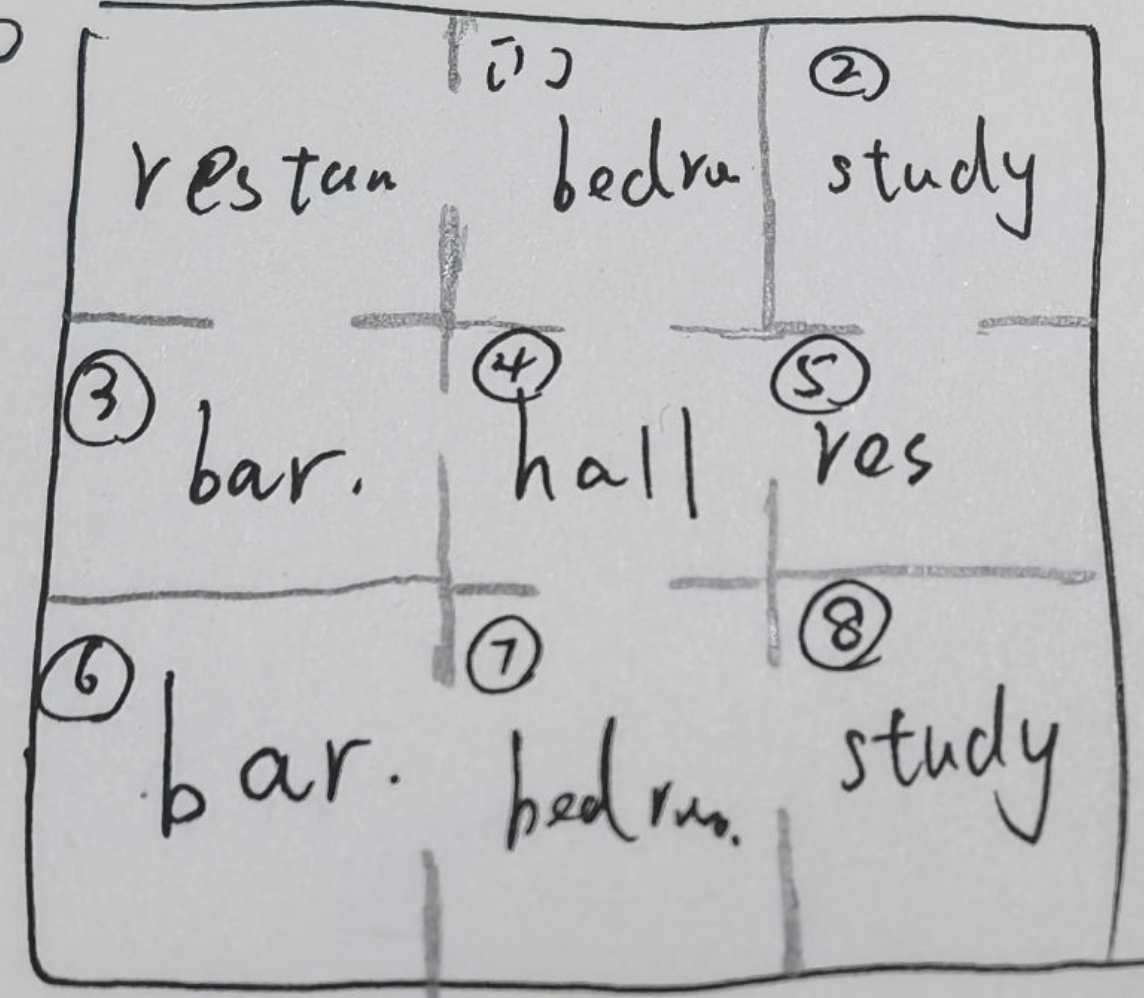
\includegraphics[width=0.7\textwidth]{1.png}
	\caption{\label{OOP3}Maze}
	\end{figure}




\end{document}